\documentclass[tikz,border=12pt]{standalone}
\usepackage[T1]{fontenc}
\usepackage{mathpazo}
\usepackage{amsmath,amssymb}
\usetikzlibrary{arrows.meta, positioning, calc}

\definecolor{stblue}{HTML}{7B97AD}
\definecolor{rwgold}{HTML}{B8995E}
\definecolor{sage}{HTML}{7A9A7E}
\definecolor{dkbrown}{HTML}{3D3530}
\definecolor{wmgray}{HTML}{7B7067}
\definecolor{cream}{HTML}{F9F6F0}
\definecolor{border}{HTML}{D4C9B8}
\definecolor{terracotta}{HTML}{C47A6A}

\begin{document}
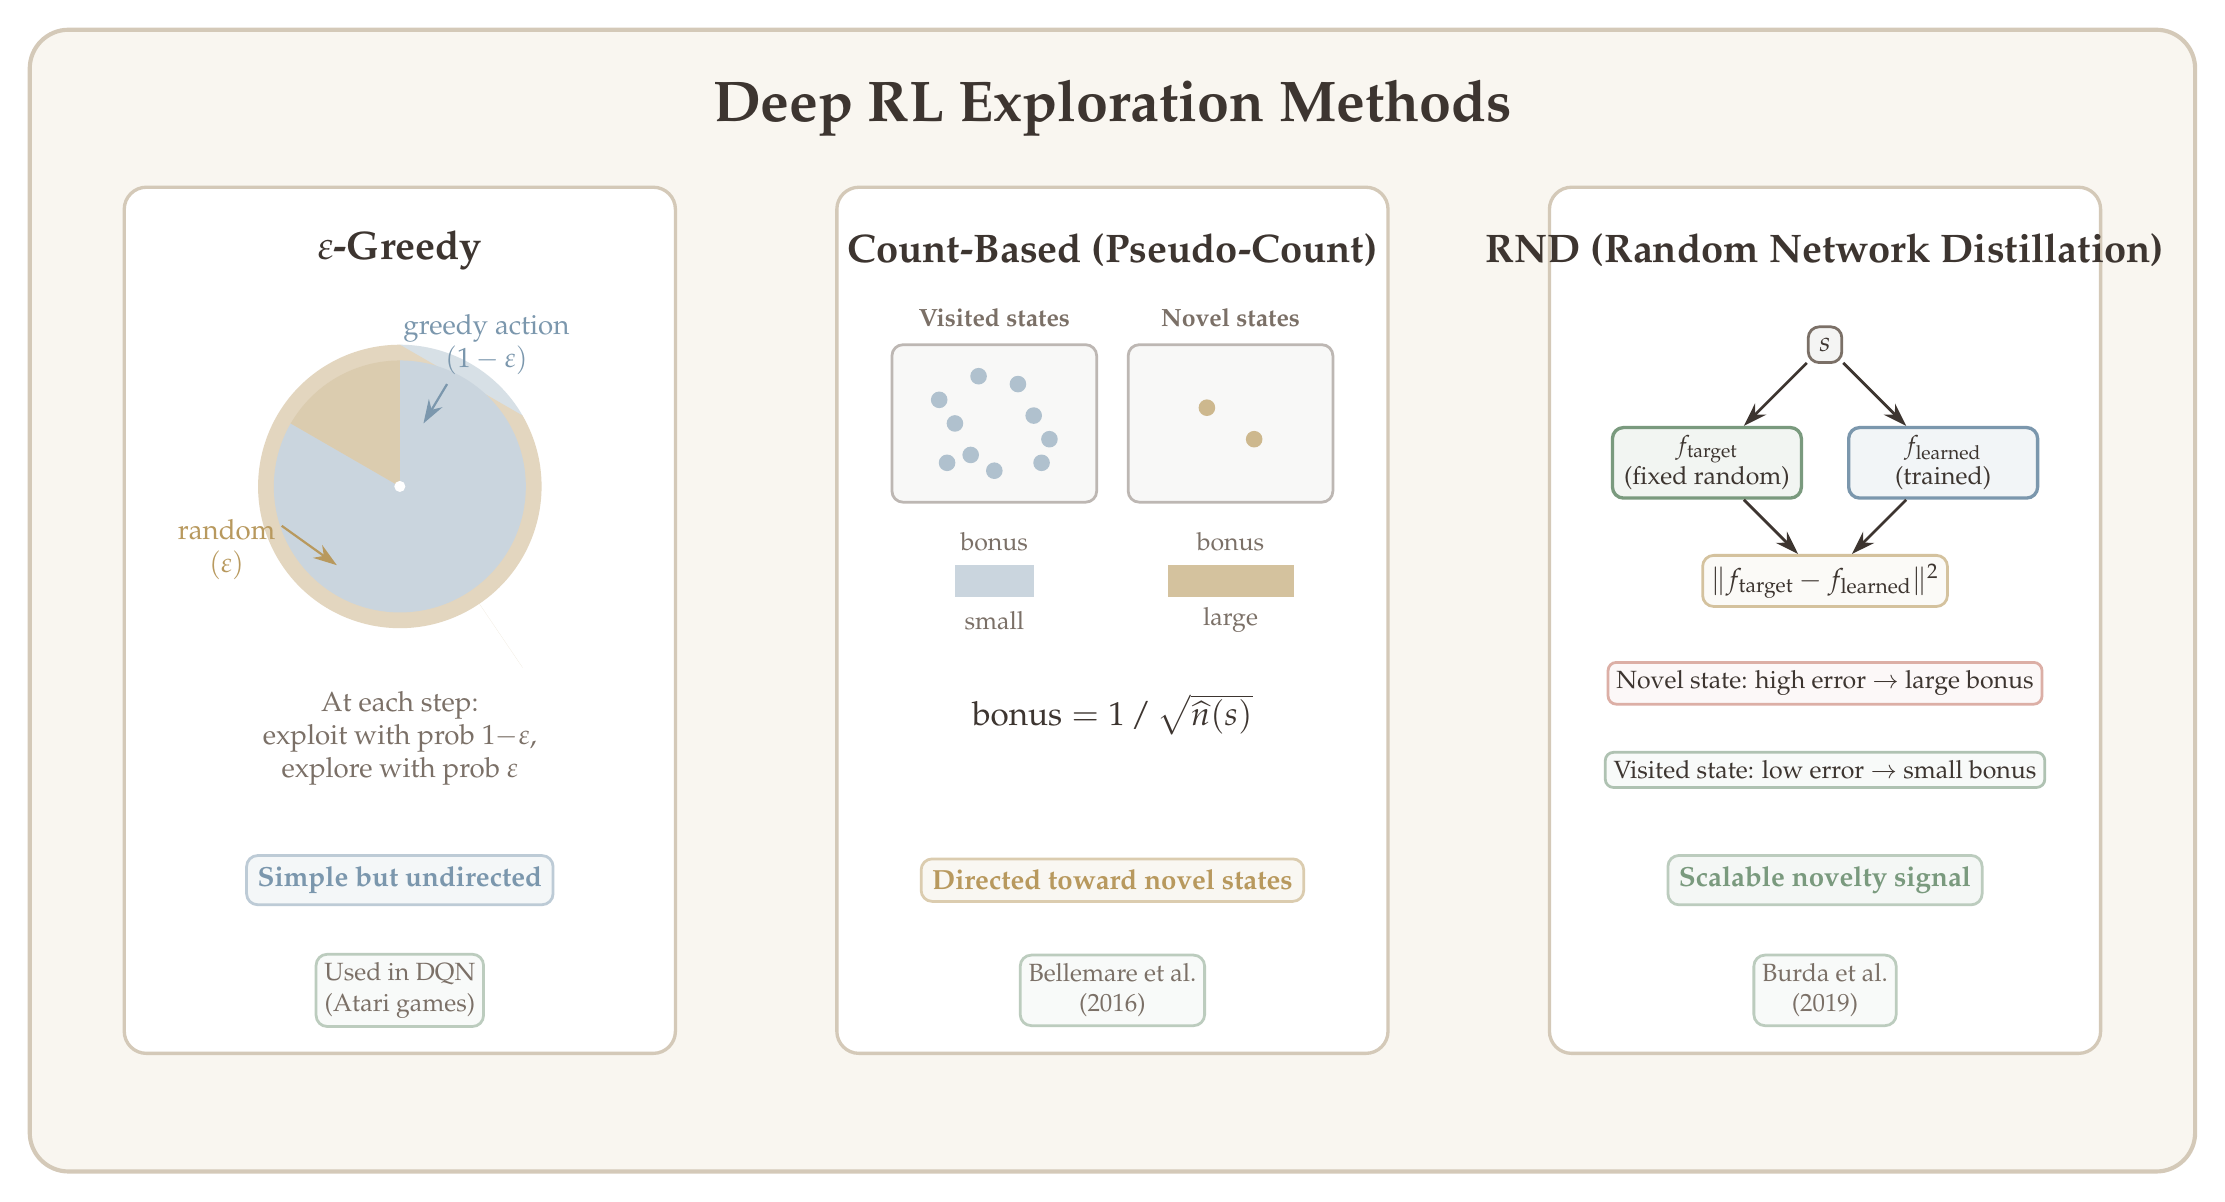
\begin{tikzpicture}[
  >={Stealth[length=3mm, width=2mm]},
]

% Background
\fill[cream, rounded corners=14pt] (-0.5,-5.5) rectangle (27,9);
\draw[border, rounded corners=14pt, line width=1.5pt] (-0.5,-5.5) rectangle (27,9);

% Title
\node[font=\huge\bfseries, text=dkbrown] at (13.25,8)
  {Deep RL Exploration Methods};

% =============================================
% Panel 1: Epsilon-Greedy
% =============================================
\begin{scope}[shift={(4.2,0)}]
\node[draw=border, line width=1.2pt, fill=white, rounded corners=8pt,
      minimum width=70mm, minimum height=110mm] at (0,1.5) {};

\node[font=\Large\bfseries, text=dkbrown] at (0,6.2) {$\varepsilon$-Greedy};

% Pie chart
\fill[stblue!30] (0,3.2) -- ++(0,1.8) arc (90:30:1.8) -- cycle;
\fill[rwgold!40] (0,3.2) -- (30:1.8)+(0,3.2) arc (30:-270:1.8) -- cycle;

% Fix pie chart position
\begin{scope}[shift={(0,3.2)}]
  \fill[stblue!40] (0,0) -- (90:1.6) arc (90:-210:1.6) -- cycle;
  \fill[rwgold!50] (0,0) -- (-210:1.6) arc (-210:-270:1.6) -- cycle;
  \fill[white] (0,0) circle (2pt);

  % Labels
  \node[font=\normalsize, text=stblue, align=center] at (1.1,1.8)
    {greedy action\\$(1 - \varepsilon)$};
  \draw[stblue, line width=0.8pt, ->] (0.6,1.3) -- (0.3,0.8);

  \node[font=\normalsize, text=rwgold, align=center] at (-2.2,-0.8)
    {random\\$(\varepsilon)$};
  \draw[rwgold, line width=0.8pt, ->] (-1.5,-0.5) -- (-0.8,-1.0);
\end{scope}

\node[font=\normalsize, text=wmgray, align=center] at (0,0)
  {At each step:\\exploit with prob $1{-}\varepsilon$,\\explore with prob $\varepsilon$};

\node[draw=stblue!50, line width=1pt, fill=stblue!8, rounded corners=4pt,
      font=\normalsize\bfseries, text=stblue, inner sep=4pt]
  at (0,-1.8) {Simple but undirected};

\node[draw=sage!50, line width=1pt, fill=sage!5, rounded corners=4pt,
      font=\small, text=wmgray, inner sep=3pt, align=center]
  at (0,-3.2) {Used in DQN\\(Atari games)};
\end{scope}

% =============================================
% Panel 2: Count-Based (Pseudo-Count)
% =============================================
\begin{scope}[shift={(13.25,0)}]
\node[draw=border, line width=1.2pt, fill=white, rounded corners=8pt,
      minimum width=70mm, minimum height=110mm] at (0,1.5) {};

\node[font=\Large\bfseries, text=dkbrown] at (0,6.2) {Count-Based (Pseudo-Count)};

% Visited states box
\node[draw=wmgray!50, line width=1pt, fill=wmgray!5, rounded corners=4pt,
      minimum width=26mm, minimum height=20mm] (visited) at (-1.5,4) {};
\node[font=\small\bfseries, text=wmgray, above] at (-1.5,5.1) {Visited states};
% Dots (many)
\foreach \x/\y in {-2.2/4.3, -1.8/3.6, -1.2/4.5, -0.8/3.8, -2.0/4.0, -1.5/3.4, -1.0/4.1, -1.7/4.6, -2.1/3.5, -0.9/3.5} {
  \fill[stblue!60] (\x, \y) circle (3pt);
}

% Novel states box
\node[draw=wmgray!50, line width=1pt, fill=wmgray!5, rounded corners=4pt,
      minimum width=26mm, minimum height=20mm] (novel) at (1.5,4) {};
\node[font=\small\bfseries, text=wmgray, above] at (1.5,5.1) {Novel states};
% Dots (few)
\foreach \x/\y in {1.2/4.2, 1.8/3.8} {
  \fill[rwgold!70] (\x, \y) circle (3pt);
}

% Bonus bars
\node[font=\small, text=wmgray] at (-1.5,2.5) {bonus};
\fill[stblue!40] (-2,1.8) rectangle (-1,2.2);
\node[font=\small, text=wmgray] at (-1.5,1.5) {small};

\node[font=\small, text=wmgray] at (1.5,2.5) {bonus};
\fill[rwgold!60] (0.7,1.8) rectangle (2.3,2.2);
\node[font=\small, text=wmgray] at (1.5,1.5) {large};

% Formula
\node[font=\large, text=dkbrown] at (0,0.3)
  {$\text{bonus} = 1 \,/\, \sqrt{\widehat{n}(s)}$};

\node[draw=rwgold!50, line width=1pt, fill=rwgold!8, rounded corners=4pt,
      font=\normalsize\bfseries, text=rwgold, inner sep=4pt]
  at (0,-1.8) {Directed toward novel states};

\node[draw=sage!50, line width=1pt, fill=sage!5, rounded corners=4pt,
      font=\small, text=wmgray, inner sep=3pt, align=center]
  at (0,-3.2) {Bellemare et al.\\(2016)};
\end{scope}

% =============================================
% Panel 3: RND
% =============================================
\begin{scope}[shift={(22.3,0)}]
\node[draw=border, line width=1.2pt, fill=white, rounded corners=8pt,
      minimum width=70mm, minimum height=110mm] at (0,1.5) {};

\node[font=\Large\bfseries, text=dkbrown] at (0,6.2) {RND (Random Network Distillation)};

% State input
\node[draw=wmgray, line width=1pt, fill=wmgray!8, rounded corners=4pt,
      font=\normalsize, text=dkbrown, inner sep=4pt]
  (rnd-s) at (0,5) {$s$};

% Two networks
\node[draw=sage, line width=1.2pt, fill=sage!10, rounded corners=4pt,
      font=\small, text=dkbrown, align=center, inner sep=3pt,
      minimum width=24mm]
  (ftgt) at (-1.5,3.5) {$f_{\text{target}}$\\(fixed random)};
\node[draw=stblue, line width=1.2pt, fill=stblue!10, rounded corners=4pt,
      font=\small, text=dkbrown, align=center, inner sep=3pt,
      minimum width=24mm]
  (fpred) at (1.5,3.5) {$f_{\text{learned}}$\\(trained)};

\draw[->, line width=1pt, dkbrown] (rnd-s) -- (ftgt);
\draw[->, line width=1pt, dkbrown] (rnd-s) -- (fpred);

% Error box
\node[draw=rwgold!60, line width=1pt, fill=rwgold!5, rounded corners=4pt,
      font=\normalsize, text=dkbrown, inner sep=3pt]
  (err) at (0,2)
  {$\|f_{\text{target}} - f_{\text{learned}}\|^2$};

\draw[->, line width=1pt, dkbrown] (ftgt) -- (err);
\draw[->, line width=1pt, dkbrown] (fpred) -- (err);

% Novel vs visited (stacked vertically to avoid overlap)
\node[draw=terracotta!60, line width=1pt, fill=terracotta!5, rounded corners=3pt,
      font=\small, text=dkbrown, align=center, inner sep=3pt]
  at (0,0.7) {Novel state: high error $\to$ large bonus};
\node[draw=sage!60, line width=1pt, fill=sage!5, rounded corners=3pt,
      font=\small, text=dkbrown, align=center, inner sep=3pt]
  at (0,-0.4) {Visited state: low error $\to$ small bonus};

\node[draw=sage!50, line width=1pt, fill=sage!8, rounded corners=4pt,
      font=\normalsize\bfseries, text=sage, inner sep=4pt]
  at (0,-1.8) {Scalable novelty signal};

\node[draw=sage!50, line width=1pt, fill=sage!5, rounded corners=4pt,
      font=\small, text=wmgray, inner sep=3pt, align=center]
  at (0,-3.2) {Burda et al.\\(2019)};
\end{scope}

\end{tikzpicture}
\end{document}
